\chapter{Einführung}
%
Ausgehend von ökonomischen, informationstechnologischen und marktpolitischen Einschnitten in den
vergangenen Jahrzehnten\footnote{Als Gründe zu nennen wären hier: die Explosion der Zeitschriftenpreise im Bereich der
Science, Technology \& Medicine (STM), das Aufkommen von E-Publishing und die Konzentration auf wenige
Verlage},
sind Bibliotheken dazu veranlasst, ihr Budget hinsichtlich der Informationsbedarfe
ihrer Nutzer:innen behutsamer zu planen und sich in zunehmenden Maße gegenüber ihren Unterhaltsträgern zu rechtfertigen.

Die Relevanz von bibliothekarischen Kennzahlen ist in diesem Zusammenhang größer geworden.
Deswegen ist es wichtig, Daten aus bibliothekarischen Servicedienstleistungen und Geschäfts-prozessen zu aggregieren, zu erheben und statistisch
auszuwerten, um auf Basis der daraus erzielten Erkenntnisse handeln zu können.

Ziel der zu entstehenden Arbeit ist die Entwicklung einer
interaktiven Business-Intelligence-Applikation als proof-of-concept,
mit der systematisch die relevanten Daten einer hybriden Spezialbibliothek aggregiert, statistisch
analysiert und mit geeigneten und modernen Datenvisualisierungstechniken\footnote{Visualisierungen können komplexe Sachverhalte herunterbrechen und
so große Datenmengen - im Gegensatz zu großen Tabellen - leicht verständlich
darstellen. Im Kontext dieser Arbeit konzentriere ich mich auf Ansätze, die Visualisierungen mittels Visualisierungstechniken algorithmisch aus
Daten erzeugen (Informationsvisualisierung, Datenvisualisierung und visuelle Analyse).\cite{RN100}}
ausgegeben werden sollen.
Vor allem soll sich hier auf automatisierte Prozesse zur Gewinnung der Ergebnisse konzentriert werden.

Mit diesen automatisch angefertigten statistischen Datenanalysen sollen zukünftige
Entscheidungen im Bibliotheksmanagement wie Erwerbungspolitik, Budgetplanung und
Mittelallokation hinsichtlich der weiteren Entwicklung der
Servicedienstleistungen evidenzbasiert und datengetrieben unterstützt werden.

Darüber hinaus soll die Applikation  eine Funktion beinhalten, ausgewählte
Resultate automatisiert als \textit{factsheet} zu exportieren, um diese
als Rechenschaftsbericht gegenüber Stakeholdern der Bibliothek präsentieren zu können.

Die Notwendigkeit für diese Applikation ist durch das
Fehlen eines zentralen Nachweisortes für bibliothekarische
Statistiken in der Bibliothek gegeben. Da die Bibliothek zudem verschiedene Recherche-Systeme den
Wissenschaftler:innen anbietet, wäre eine Engführung der statistischen
Datenerhebung auf eine Plattform begrüßenswert.
Des Weiteren ist das Erfordernis, bibliothekarische Geschäftsprozesse zu evaluieren und die
Servicedienstleistungen bezüglich der Ziele der Institution noch weiter zu
optimieren, von großer Relevanz. Mit dem Ende der Konsolidierungsphase der
Bibliothek, die im Zuge des \textit{Max-Planck-Institutes für empirische
Ästhetik} 2014 gegründet wurde, tritt sie ein in eine Phase, in der ab dem Jahr
2021 Budgetplanungen eine größere Rolle spielen werden.

Die zu entstehende Applikation könnte hierbei helfen, systematisches Controlling einzuführen und das
Bibliotheksmanagement weiter zu professionalisieren.
%predictive analysis\\
Um künftigen Anforderungen gewachsen zu sein, soll sie
modulbasiert programmiert werden und dadurch leicht erweiterbar und eventuell von
anderen Bibliotheken nachnutzbar sein.
%evidence based stock management\\

%Erschaffen eines Reports

\section{Problemstellung}
Die Bibliothek des \textit{Max-Planck-Institutes für empirische Ästhetik}
ist Teil des \textit{hessischen Bibliotheksverbundes (HeBis)}. Die Geschäftsprozesse
der Katalogisierung und der Erwerbung finden im Zentralsystem \textit{CBS} und im im Lokalsystem \textit{LBS4} von
\textit{OCLC} statt. \textit{LBS4} wird gehostet und betreut vom Lokalsystem-Team Frankfurt. Als Service-Leistung werden der Bibliothek besondere Funktionalitäten
für das \textit{CBS} bereitgestellt. Außerdem erhält die Bibliothek unter anderem Ausleih-, Budget- und
Umsatzübersichten als Text per E-Mail zugesandt.


Neben der Verankerung in der deutschen Bibliotheksverbundlandschaft
wird die Bibliothek in ihren Aufgaben von der
\textit{Max Planck Digital Library (mpdl)}
unterstützt. Deren Portfolio umfasst vorrangig die zentrale Lizenzierung
von relevanten elektronischen Informationsressourcen, die Bereitstellung
von Softwarelösungen, das Betreiben eines Publikationsrepositoriums und
das Vorantreiben von Open-Access. Zudem stellt sie den Bibliotheken der einzelnen Max-Planck-Institute
\textit{COUNTER}-Statistiken zur Verfügung, die von den Verlagen geliefert werden.

Außer diesen bereitgestellten Daten erhebt die Bibliothek Daten unter anderem über
die Frequentation des Lesesaals, die Nutzung des nehmenden Fernleihservices, des
Dokumentenlieferdienstes \textit{subito} und des Bestandswachstums vor Ort.
Nach den unterschiedlichen Verantwortlichkeiten aufgeteilt, werden diese Daten an verschiedenen virtuellen Orten erhoben.
Eine systematische Auswertung der Daten findet nur unzureichend statt.
Daher regt sich der Wunsch seitens der Bibliotheksleitung und der Mitarbeiter:innen nach einem gemeinsamen Tool,
mit dem übersichtlich und klar alle notwendigen nutzungs- und sammlungsbezogenen Statistiken einer
Spezialbibliothek erfasst und dargestellt werden können.\footnote{Zwar führt \textit{HeBis} eine Bestandsstatistik, diese ist aber insbesondere für die
Evaluation und Optimierung von Geschäftsprozessen einer Spezialbibliothek
insuffizient. \url{https://www.hebis.de/de/1ueber_uns/statistik/cbs_statistik.php} Auch an der deutschen Bibliotheksstatistik nimmt die Bibliothek nicht teil. Beide bieten zudem nur Zahlenkolonnen und keine weiteren Visualisierungen an.}

In der  \autoref{tab:Geschäftsgänge} werden die Geschäftsgänge aufgezeigt, zu denen statistische Daten
in der Bibliothek erhoben bzw. von verschiedenen Anbietern zur Verfügung gestellt werden. Im folgenden wird sich auf folgende
Geschäftsgänge konzentriert.
Außer diesen bereitgestellten Daten erhebt die Bibliothek Daten unter anderem über
die Frequentation des Lesesaals, die Nutzung des nehmenden Fernleihservices, des
Dokumentenlieferdienstes \textit{subito} und des Bestandswachstums vor Ort.

In der  \autoref{tab:Geschäftsgänge} werden die Geschäftsgänge aufgezeigt, zu denen statistische Daten
in der Bibliothek erhoben bzw. von verschiedenen Anbietern zur Verfügung gestellt werden. Im folgenden wird sich auf folgende
Geschäftsgänge konzentriert.
Außer diesen bereitgestellten Daten erhebt die Bibliothek Daten unter anderem über
die Frequentation des Lesesaals, die Nutzung des nehmenden Fernleihservices, des
Dokumentenlieferdienstes \textit{subito} und des Bestandswachstums vor Ort.

\begin{table}[h]
    \centering
    \begin{adjustbox}{max width=\textwidth}
    \begin{tabular}{llll}
       \toprule
       \textbf{Geschäftsgang}& \textbf{erhobene Daten} & \textbf{Format} & \textbf{Quelle}\\
       \midrule     
            Buchservice              & Fernleihe                            & Excel  & eigenständig \\ 
            Buchservice              & Scan                                 & Excel  & eigenständig \\ 
            Buchservice              & Subito                               & Excel  & eigenständig \\ 
            Buchservice              & Sonstiges                            & Excel  & eigenständig \\ 
            Buchservice              & elektronisch                         & Excel  & eigenständig \\ 
            Buchservicw              & Ausleihen pro Abteilung              & Excel  & eigenständig \\ 
            Bibliotheksbenutzung     & Benutzer:Innenanzahl                 & Excel  & eigenständig \\ 
            Bibliotheksbenutzung     & nachgefragte Medien                  & email  & LBS          \\ 
            Ausleihe                 & Ausleihstatistik                     & Excel  & LBS          \\ 
            Erwerbung                & monatliche Ausgaben nach Lieferanten & email  & LBS          \\ 
            Erwerbung                & Budgetübersicht nach Kostenstellen   & email  & LBS          \\ 
            Bucheingang              & monatliche Neuerwerbungslisten       & Word   & LBS          \\ 
            Elektronische Ressourcen & Counter-Statistiken                  & tsv    & mpdl         \\ 
            Bestand                  & eigene                               & csv    & LBS          \\
        \bottomrule
    \end{tabular}
    \end{adjustbox}
    \caption
    \end{table}


Nach den unterschiedlichen Verantwortlichkeiten aufgeteilt, werden diese Daten an verschiedenen virtuellen Orten erhoben.
Eine systematische Auswertung der Daten findet nur unzureichend statt.
Außer diesen bereitgestellten Daten erhebt die Bibliothek Daten unter anderem über
die Frequentation des Lesesaals, die Nutzung des nehmenden Fernleihservices, des
Dokumentenlieferdienstes \textit{subito} und des Bestandswachstums vor Ort.

Im Data-Science-Cycle wird wie folgt der Vorgang beschrieben. Dabei fallen ungefähr 60 \% des Aufwandes auf die Bereinigung der Daten. 
Weniger Aufwändig dagegen ist die Datenvisualisierung.



Nach den unterschiedlichen Verantwortlichkeiten aufgeteilt, werden diese Daten an verschiedenen virtuellen Orten erhoben.
Eine systematische Auswertung der Daten findet nur unzureichend statt.
Außer diesen bereitgestellten Daten erhebt die Bibliothek Daten unter anderem über
die Frequentation des Lesesaals, die Nutzung des nehmenden Fernleihservices, des
Dokumentenlieferdienstes \textit{subito} und des Bestandswachstums vor Ort.

In der \autoref{fig:data science} wird wie folgt der Vorgang beschrieben. Dabei fallen ungefähr 60 \% des Aufwandes auf die Bereinigung der Daten. 
Weniger Aufwändig dagegen ist die Datenvisualisierung

\begin{figure}[h]
    \centering
        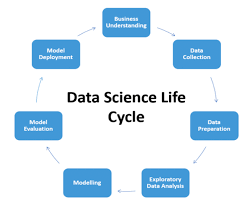
\includegraphics[width=8cm]{ds_cycle}
        \caption{Data Science Cycle}
        \label{fig:data science}
\end{figure}



Im Data-Science-Cycle wird wie folgt der Vorgang beschrieben. Dabei fallen ungefähr 60 \% des Aufwandes auf die Bereinigung der Daten. 
Weniger Aufwändig dagegen ist die Datenvisualisierung.

Nach den unterschiedlichen Verantwortlichkeiten aufgeteilt, werden diese Daten an verschiedenen virtuellen Orten erhoben.
Eine systematische Auswertung der Daten findet nur unzureichend statt.
Außer diesen bereitgestellten Daten erhebt die Bibliothek Daten unter anderem über
die Frequentation des Lesesaals, die Nutzung des nehmenden Fernleihservices, des
Dokumentenlieferdienstes \textit{subito} und des Bestandswachstums vor Ort.

Im Data-Science-Cycle wird wie folgt der Vorgang beschrieben. Dabei fallen ungefähr 60 \% des Aufwandes auf die Bereinigung der Daten. 
Weniger Aufwändig dagegen ist die Datenvisualisierung.